\chapter{Intel RealSense Depth Camera D435}
\label{cap:realsense-d435}

Este \gls{tfg} se enmarca en un proyecto que utiliza la cámara \gls{rgbd} Intel RealSense Depth Camera D435, por lo que aquí se explica el funcionamiento de esta.

Intel RealSense Depth Camera D435 es un sensor \gls{rgbd} de propósito general. 
Este sensor \gls{3d} tiene una profundidad mínima de 0,2 metros y escanea entornos de hasta 10 metros de ancho con una profundidad de resolución de hasta 1280x720 a 90 fotogramas por segundo (fps).
El sistema utiliza un procesador Intel D4vision de 28 nanómetros para procesar datos de profundidad complejos en tiempo real y un procesador de imágenes en color Realtek.
El proyector láser \gls{ir} mide solo 2,7x1,8 milímetros, utiliza tecnología \gls{vcsel} y puede grabar 60 fps.
El dispositivo RealSense D435 tiene tres sensores para capturar la imagen: un sensor CMOS 1080p RGB para capturar imágenes con color y dos sensores de 1 megapíxel a los lados izquierdo y derecho del sensor \gls{ir} \gls{vcsel}.
Estos dos últimos sensores son utilizados para obtener las imágenes en profundidad mediante una tecnología estéreo activa.
El sensor es capaz de proporcionar imágenes de alta definición gracias al procesador de visión, el proyector \gls{vcsel} y el sensor de imagen.
En la Figura \ref{fig:d435-sensors2} podemos ver los sensores descritos en el Intel RealSense D435.

\begin{figure}[h]
    \centering
    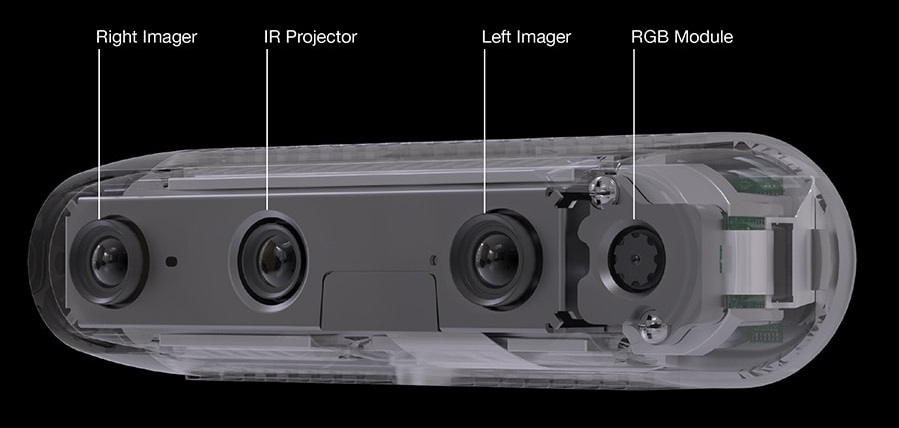
\includegraphics[width=0.7\textwidth]{archivos/d435_sensors.jpg}
    \caption{Sensores Intel RealSense D435.}
    \label{fig:d435-sensors2}
\end{figure}

La tecnología estéreo activa, o ``Active Stereo'' en inglés, funciona por triangulación.
El sensor puede ver el mismo punto desde dos ubicaciones diferentes, desde el sensor de 1 megapíxel ubicado a la izquierda del sensor \gls{vcsel} y desde el sensor de 1 megapíxel ubicado a la derecha.
Con esta información puede usar la trigonometría para medir la distancia real que hay desde el sensor hasta el punto.
Tras identificar un punto común en ambas imágenes, usa el ángulo conocido de cada sensor para cada imagen y la distancia entre ambos sensores para calcular la distancia.
Para ello, el sensor tiene un calibrado interno sobre el ángulo y distancia de ambos sensores.
Cuanto más larga es la distancia entre los sensores de imagen, más precisa es la medición.
En la Figura \ref{fig:ejemplo-sensor-estereo-activo} podemos ver un ejemplo donde para un punto común, conociendo el ángulo 'a' y 'b', y la distancia entre los sensores, se puede calcular la distancia al punto común.

\begin{figure}[h]
    \centering
    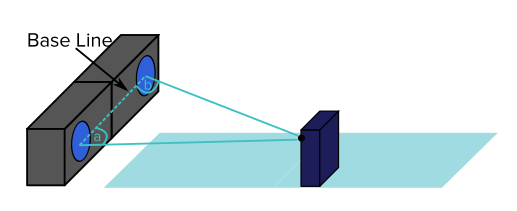
\includegraphics[width=0.7\textwidth]{archivos/ejemplo-sensor-estereo-activo.png}
    \caption{Ejemplo de identificación de un punto común con tecnología estéreo activa. Figura extraída de \cite{rafaelWhyte}.}
    \label{fig:ejemplo-sensor-estereo-activo}
\end{figure}

Con la tecnología estéreo activa, es importante hacer coincidir las mismas características en ambas imágenes.
Una forma de mejorar esto es proyectar patrones de puntos, cada sensor de profundidad puede identificar cada punto único.
De esta forma, la proyección de puntos facilita la coincidencia de características y permite medir objetos sin características, como paredes blancas.

El D435 utiliza la combinación de estéreo activo y pasivo, por lo que puede medir objetos más cercanos sin rasgos distintivos y objetos más lejanos.
